%File: formatting-instruction.tex
\documentclass[letterpaper]{article}
\usepackage{aaai}
\usepackage{times}
\usepackage{helvet}
\usepackage{courier}
\usepackage{graphicx}
\frenchspacing
\setlength{\pdfpagewidth}{8.5in}
\setlength{\pdfpageheight}{11in}
\pdfinfo{
/Title (Baewatch:\\regola di voto per un sistema di raccomandazione di gruppo\\in contesto multiagente collaborativo)
/Author (Alessandro Pasqualini)}
\setcounter{secnumdepth}{0}  
 \begin{document}
% The file aaai.sty is the style file for AAAI Press 
% proceedings, working notes, and technical reports.
%
\title{Baewatch:\\regola di voto per un sistema di raccomandazione di gruppo\\in contesto multiagente collaborativo}
\author{Alessandro Pasqualini\\
Dipartimento di Ingegneria dell'Informazione\\
Università di Padova, Padova\\
alessandro.pasqualini@studenti.unipd.it\\
}
\maketitle
\begin{abstract}
\begin{quote}
Al giorno d'oggi i sistemi di raccomandazione veicolano la scelte degli utenti in moltissimi settori, accumulando conoscenza sulle loro preferenze. Queste preferenze sono successivamente elaborate da specifici algoritmi per predire e consigliare all'utente il suo prossimo acquisto, il prossimo film da vedere, etc. Le informazioni ottenute sono incrociate con quelle di altri utenti migliorandone l'accuratezza.

Una delle sfide più importanti è quella di utilizzare le preferenze dei vari utenti per ottenere delle raccomandazioni di gruppo, dove è necessario soddisfare interessi differenti e a volte contrastanti tra di loro. In questo contento nasce Baewatch, una regola di voto il cui scopo è selezionare una raccomandazione per il gruppo in modo da massimizzate la "contentezza" di ogni componente.

\end{quote}
\end{abstract}

\section{Introduzione}
Internet ha assunto negli anni un ruolo sempre più centrale nella vita quotidiana, arrivando a diventare uno dei principali mercati dove poter acquistare un numero sempre maggiore di beni. Il numero esponenziale di possibilità di acquisto ha spinto lo sviluppo e la realizzazione di sistemi di raccomandazione in modo da consigliare ed aiutare l'utente nella scelta.

All'interno di alcuni settori, ad esempio lo streaming di film e serie tv, questi sistemi si sono rivelati essenziali per il successo di alcuni dei principali player. Netflix, Amazon, Google devono parte del loro successo commerciale a questi algoritmi, tanto che sono parte essenziale della loro offerta.

\begin{figure}[!htb]
    \begin{centering}
        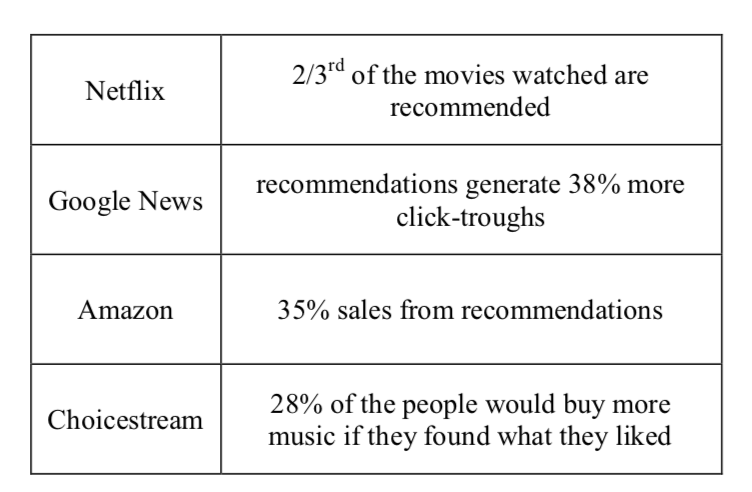
\includegraphics[width=\linewidth]{Figures/successo.png}
        \caption{Successo dei sistemi di raccomandazione di alcune piattaforme \cite{ref1}}
        \label{fig:successo}
    \end{centering}
\end{figure}

Le raccomandazioni fornite dai sistemi di raccomandazioni possono essere accettate oppure ignorate da parte dell'utente. Le interazioni, dirette o indirette, che l'utente ha nei confronti di quanto consigliato dal sistemi formano un insieme di informazioni che sono utilizzate dallo stesso sistema di raccomandazione per migliorare la sua qualità in futuro.

Questi sistemi possono sfruttare modelli, quali il collaborative filtering in modo da incrociare le informazioni di altri utenti ritenuti simili, secondo qualche metrica, per assegnare una valutazione ad un bene non ancora acquistato dall'utente.

Una delle principali sfide dei sistemi di raccomandazione è fornire delle raccomandazioni per gruppi di utenti, bilanciando bisogni e scelte differenti dei vari membri. Un esempio è proprio la raccomandazione di un film ad un gruppo di persone: in questo contesto è possibile riconoscere alcune difficoltà non presenti nel contesto individuale. Alcuni membri del gruppo potrebbero avere interessi competitivi e sarà l'intero gruppo ad accettare o rifiutare la proposta generata.

\section{Collaborative Filtering}

\section{La regola di voto Baewatch}

\section{Esempi di applicazione di Baewatch}

\section{Conclusioni}

\section{Materiale aggiuntivo}
Una prima implemnetazione in Pyhton dell'algoritmo presentato è disponibile presso https://github.com/alessandro1105/baewatch. All'interno del repository è possibile trovare il file \emph{test\_complete.py} che permette di valutare l'algoritmo utilizzando il MovieLens 100K Dataset (https://grouplens.org/datasets/movielens/100k/). Il file \emph{test\_paper.py} contiene i test cases presentati in questo documento, insieme ad altri non citati, per dimostrare l'efficacia della regola di voto.

\bigskip
\noindent Thank you for reading these instructions carefully. We look forward to receiving your electronic files!

\bibliographystyle{aaai} 
\bibliography{bibliography}

\end{document}